\chapter{Installation}
\label{chapter:Installation}

\index{Installation|textbf}

This section describes the process for installing ITK on your system. Keep in
mind that ITK is a toolkit, as such, once it is installed in your computer
there will be no application to run. Rather, you will use ITK to build your
own applications. What ITK does provide---besides the toolkit proper---is a
large set of test files and examples that will introduce you to ITK concepts
and will show you how to use ITK in your own projects.

Some of the examples distributed with ITK require third party libraries that
you may have to download. For an initial installation of ITK you may want to
ignore these extra libraries and just built the toolkit itself. In the past,
a large fraction of the traffic on the insight-users mailing list originates from
difficulties in getting third party libraries compiled and installed rather
than with actual problems building ITK.

ITK has been developed and tested across different combinations of operating
systems, compilers, and hardware platforms including MS-Windows, Linux on
Intel-compatible hardware, Solaris, IRIX and recently the Mac. Popular
compilers like Visual Studio 6.0, Visual Studio 7.0, gcc 2.95.2, gcc 2.96,
gcc 3.04, gcc 3.1, gcc 3.2, Borland 5.5 and SGI-CC 6.5 are currently
supported. Given the advanced usage of C++ features in the toolkit, some
compilers may have difficulties processing the code. If you are currently
using an outdated compiler this may be an excellent excuse for upgrading this
old piece of software!

\section{Configuring ITK}
\label{sec:ConfiguringITK}

\index{Configuration|textbf}
 
The challenge of supporting ITK across platforms has been solved through the
use of CMake, a cross-platform, open-source build system. CMake is used to
control the software compilation process using simple platform and compiler
independent configuration files.  CMake generates native makefiles and
workspaces that can be used in the compiler environment of your choice. CMake
is quite sophisticated, it supports complex environments requiring system
configuration, code pre-processing, code generation, and template
instantiation.

CMake generates Makefiles under UNIX and Cygwin systems and generates Visual
Studio workspaces under Windows (and appropriate build files for other
compilers like Borland). The information used by CMake is provided by
\code{CMakeLists.txt} files that are present in every directory of the ITK
source tree. These files contains information that the user
provides to CMake at configuration time. Typical information includes paths
to utilities in the system and the selection of software options specified by
the user.

\subsection{Preparing CMake}
\label{sec:CMakeforITK}
 
\index{CMake|textbf}
\index{CMake!downloading}

CMake can be downloaded at no cost from 
\begin{center} 
  \url{http://www.cmake.org}
\end{center}

ITK require the latest release of CMake\footnote{The current version at the
time of writing this document is CMake 1.4 patch 7.}. You can download binary
versions for most of the popular platforms including Windows, Solaris, IRIX,
HP, Mac and Linux. Alternatively you can download the source code and build
CMake on your system. It is very important to avoid having several different
versions of CMake simultaneously. The reason is that CMake searches your
system in order to find its components, and mixing components from different
versions will produce inconsistent executables. Follow the instructions in the
CMake Web page for downloading and installing the software.

Running CMake initially requires that you provide two pieces of information:
where the source code directory is located (ITK\_SOURCE\_DIR), and where the
object code is to be produced (ITK\_BINARY\_DIR). These are referred to as the
\emph{source directory} and the \emph{binary directory}. On Unix, the binary
directory is created by the user and CMake is invoked with the path to the
source directory. For example:

\begin{verbatim}
mkdir Insight-binary
cd Insight-binary
ccmake ../Insight
\end{verbatim}

Note that the source directory and the build directory can be the
same---this is known as an \emph{in-source} build. On Windows, the CMake 
GUI is used to specify the source and build directories (Figure
\ref{fig:CMakeGUI}).

CMake runs in an interactive mode in that you iteratively select options and
configure according to these options. The iteration proceeds until no more
options are selected. At this point, a generation step produced the appropriate
build files for your configuration.

This interactive configuration process can be better understood if you
imagine that you are walking through a decision tree.  Every option that you
select introduces the possibility that new, dependent options may become
relevant. These new options are presented by CMake at the top of the options
list in its interface.  Only when no new options appear after a configuration
iteration can you be sure that the necessary decisions have all been made. At
this point build files are generated for the current configuration.

\subsection{Configuring ITK}
\label{sec:ConfiguringITKwithVTK}
  
\index{Configuration!with VTK}

\begin{figure}[ht]
\centering 
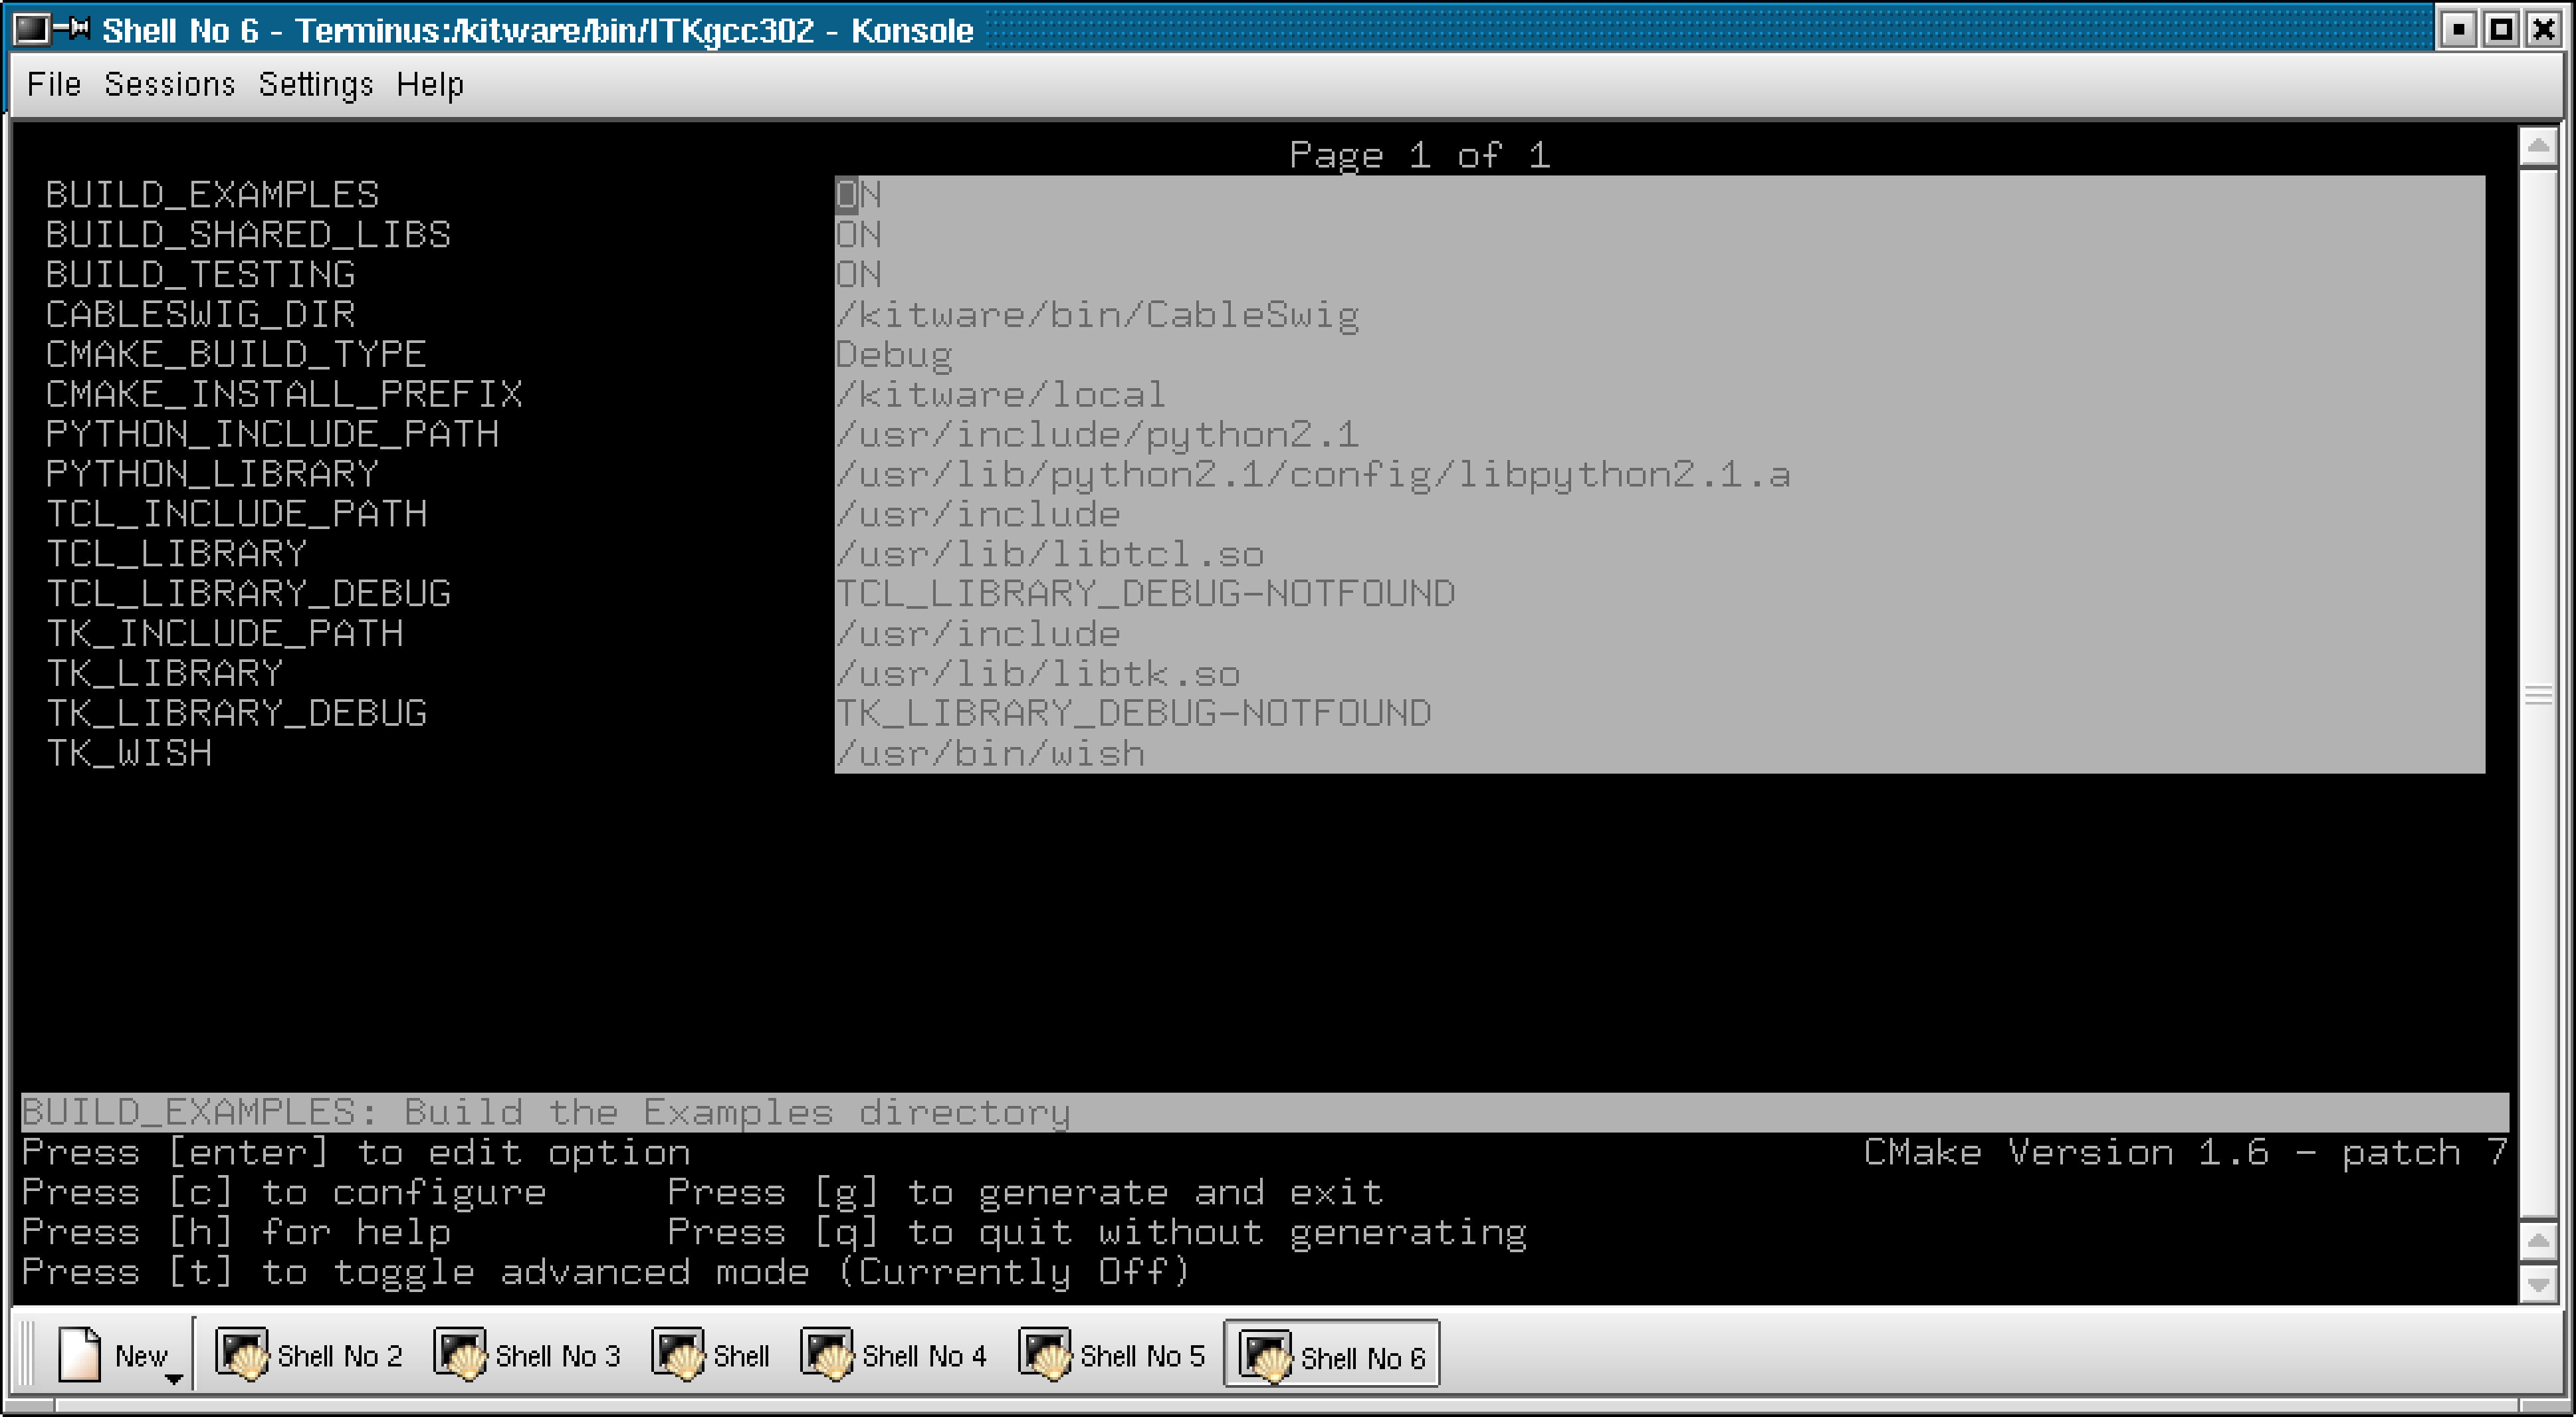
\includegraphics[height=0.45\textwidth]{ccmakeScreenShot.eps}
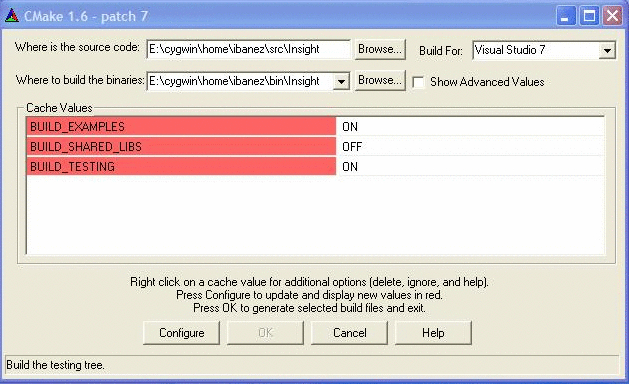
\includegraphics[height=0.45\textwidth]{CMakeSetupScreenShot.eps}
\caption[Cmake user interface]{CMake interface. Left) \texttt{ccmake}, the UNIX
version based on \texttt{curses}. Right) \texttt{CMakeSetup}, the MS-Windows
version based on MFC}
\label{fig:CMakeGUI}
\end{figure}

Figure \ref{fig:CMakeGUI} shows the CMake interface for UNIX and MS-Windows.
In order to speed up the build process and to avoid compilation problems you
may want to disable the compilation of the demo applications. This is done
with the variable
\code{BUILD\_APPLICATIONS=OFF}. The demo applications  distributed with the
toolkit are a helpful resource for learning how to write applications with
ITK.  However, due to the large number of examples and the fact that some of
them rely on third party libraries, enabling this option will considerably
complicate the initial configuration of the toolkit and is best avoided the
first time.

Begin running CMake by using \code{ccmake} on Unix, and \code{CMakeSetup} on
Windows. Remember to run \code{ccmake} from the binary directory on Unix. On
Windows, specify the source and binary directories in the GUI, then begin to
set the build variables in the GUI as necessary.  Most variables should have
default values that are sensible. Each time you change a set of variables in
CMake, it is necessary to proceed to another configuration step. In the
Windows version this is done by clicking on the ''Configure'' button. In the
UNIX version this is done in a
\code{curses} interface where you can select to configure by hitting the
''c'' key.

When no new options appear in CMake, you can proceed to generate Makefiles or
Visual Studio projects. This is done in Windows by clicking on the ''Ok''
button.  In the UNIX version this is done by hitting the ''g'' key. After the
generation process CMake will quit silently. To initiate the build process
on UNIX, simply type \code{make} in the binary directory. Under Windows, load
the workspace named \code{ITK.dsw} from the binary directory you specified
in the CMake GUI.

The build process will typically take anywhere from 30 minutes to one hour
depending on the performance of your system. As part of the normal built
process, about 300 small test programs are compiled. This verifies that the
basic components of ITK have been correctly built on your system.

\section{Getting Started With ITK }
\label{sec:GettingStartedWithITK}
 
The simplest way to create a new project with ITK is to create a new directory
somewhere in your disk and create two files in it. The first one is a
\code{CMakeLists.txt} file that will be used by CMake to generate a Makefile
(if you are using UNIX) or a Visual Studio workspace (if you are using
MS-Windows).  The second file is an actual C++ program that will exercise
some of the large number of classes available in ITK. The details of these files
are described in the following section.

Once both files are in your directory you can run CMake in order to configure
your project. Under UNIX, you can \code{cd} to your newly created directory
and type \code{"ccmake . "}. Note the "." in the command line for indicating
that the \code{CMakeLists.txt} file is in the current directory. The
\code{curses} interface will require you to provide the directory where ITK
was built. This is the same path that you indicated for the
\code{ITK\_BINARY\_DIR} variable at the time of configuring ITK. Under
Windows you can run \code{CMakeSetup} and provide your newly created
directory as being both the source directory and the binary directory for
your new project (i.e., an in-source build). Then CMake will require you to
provide the path to the binary directory where ITK was built. The ITK binary
directory will contain a file named \code{UseITK.cmake} generated during the
configuration process at the time ITK was built.  From this file, CMake will
recover all the information required to configure your new ITK project.

\subsection{Hello World !}
\label{sec:HelloWorldITK}

\index{Hello World|textbf}

Here is the content of the two files to write in your new project. These two
files can be found in the \code{Insight/Examples/Installation} directory. The
\code{CMakeLists.txt} file contains the following lines:

\begin{verbatim}
PROJECT(HelloWorld)

FIND_PACKAGE(ITK)
IF(ITK_FOUND)
  INCLUDE(${ITK_USE_FILE})
ELSE(ITK_FOUND)
  MESSAGE(FATAL_ERROR
          "ITK not found. Please set ITK_DIR.")
ENDIF(ITK_FOUND)

ADD_EXECUTABLE(HelloWorld HelloWorld.cxx )

TARGET_LINK_LIBRARIES(HelloWorld ITKCommon)
\end{verbatim}

The first line defines the name of your project as it appears in Visual
Studio (it will have no effect under UNIX). The second line loads a CMake
file with a predefined strategy for finding ITK \footnote{Similar files are
provided in CMake for other commonly used libraries, all of them named
\code{Find*.cmake}}. If the strategy for finding ITK fails, CMake will prompt
you for the directory where ITK is installed in your system. In that case you
will write this information in the \code{ITK\_BINARY\_DIR} variable. The line \code{
INCLUDE(\${USE\_ITK\_FILE})} loads the \code{UseITK.cmake} file containing
all the configuration information from ITK. The \code{LINK\_LIBRARIES} line
specify which ITK libraries will be linked against this project. Finally the
line
\code{ADD\_EXECUTABLE} defines as its first argument the name of the executable
that will be produced as result of this project. The remaining arguments of
\code{ADD\_EXECUTABLE} are the names of the source files to be compiled and linked.

\input HelloWorld.tex

At this point you have successfully installed and compiled ITK, and created
your first simple program. If you have difficulties, please join the
insight-users mailing list (Section \ref{sec:JoinMailList} on page
\pageref{sec:JoinMailList}) and pose questions there.
